% Created by tikzDevice version 0.12.6 on 2025-03-31 13:45:14
% !TEX encoding = UTF-8 Unicode
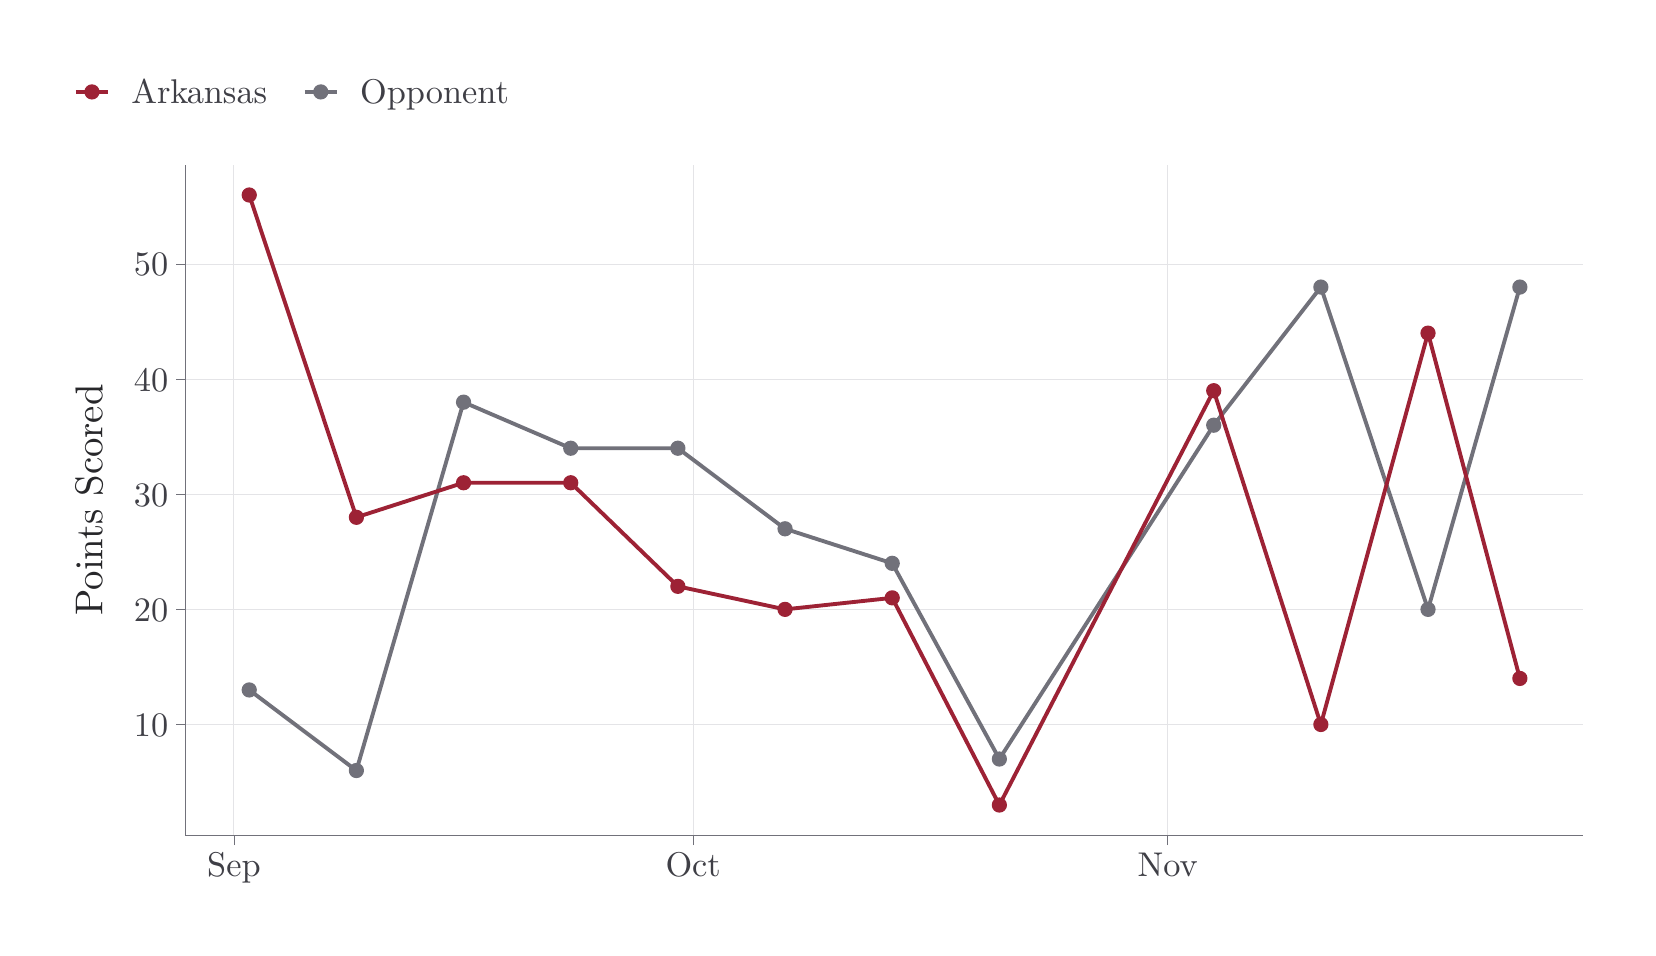
\begin{tikzpicture}[x=1pt,y=1pt]
\definecolor{fillColor}{RGB}{255,255,255}
\path[use as bounding box,fill=fillColor] (0,0) rectangle (578.16,325.21);
\begin{scope}
\path[clip] (  0.00,  0.00) rectangle (578.16,325.21);
\definecolor{drawColor}{RGB}{255,255,255}

\path[draw=drawColor,line width= 0.7pt,line join=round,line cap=round,fill=fillColor] (  0.00,  0.00) rectangle (578.16,325.21);
\end{scope}
\begin{scope}
\path[clip] ( 57.10, 33.29) rectangle (562.16,275.76);
\definecolor{drawColor}{RGB}{255,255,255}
\definecolor{fillColor}{RGB}{255,255,255}

\path[draw=drawColor,line width= 0.7pt,line join=round,line cap=round,fill=fillColor] ( 57.10, 33.29) rectangle (562.16,275.76);
\definecolor{drawColor}{RGB}{228,228,231}

\path[draw=drawColor,line width= 0.4pt,line join=round] ( 57.10, 73.42) --
	(562.16, 73.42);

\path[draw=drawColor,line width= 0.4pt,line join=round] ( 57.10,115.01) --
	(562.16,115.01);

\path[draw=drawColor,line width= 0.4pt,line join=round] ( 57.10,156.60) --
	(562.16,156.60);

\path[draw=drawColor,line width= 0.4pt,line join=round] ( 57.10,198.19) --
	(562.16,198.19);

\path[draw=drawColor,line width= 0.4pt,line join=round] ( 57.10,239.78) --
	(562.16,239.78);

\path[draw=drawColor,line width= 0.4pt,line join=round] ( 74.53, 33.29) --
	( 74.53,275.76);

\path[draw=drawColor,line width= 0.4pt,line join=round] (240.48, 33.29) --
	(240.48,275.76);

\path[draw=drawColor,line width= 0.4pt,line join=round] (411.97, 33.29) --
	(411.97,275.76);
\definecolor{drawColor}{RGB}{113,113,122}

\path[draw=drawColor,line width= 1.4pt,line join=round] ( 80.06, 85.90) --
	(118.78, 56.78) --
	(157.50,189.88) --
	(196.23,173.24) --
	(234.95,173.24) --
	(273.67,144.13) --
	(312.40,131.65) --
	(351.12, 60.94) --
	(428.57,181.56) --
	(467.29,231.47) --
	(506.01,115.01) --
	(539.20,231.47);
\definecolor{fillColor}{RGB}{113,113,122}

\path[draw=drawColor,line width= 0.5pt,line join=round,line cap=round,fill=fillColor] (467.29,231.47) circle (  2.50);

\path[draw=drawColor,line width= 0.5pt,line join=round,line cap=round,fill=fillColor] (428.57,181.56) circle (  2.50);

\path[draw=drawColor,line width= 0.5pt,line join=round,line cap=round,fill=fillColor] (196.23,173.24) circle (  2.50);

\path[draw=drawColor,line width= 0.5pt,line join=round,line cap=round,fill=fillColor] ( 80.06, 85.90) circle (  2.50);

\path[draw=drawColor,line width= 0.5pt,line join=round,line cap=round,fill=fillColor] (273.67,144.13) circle (  2.50);

\path[draw=drawColor,line width= 0.5pt,line join=round,line cap=round,fill=fillColor] (157.50,189.88) circle (  2.50);

\path[draw=drawColor,line width= 0.5pt,line join=round,line cap=round,fill=fillColor] (118.78, 56.78) circle (  2.50);

\path[draw=drawColor,line width= 0.5pt,line join=round,line cap=round,fill=fillColor] (351.12, 60.94) circle (  2.50);

\path[draw=drawColor,line width= 0.5pt,line join=round,line cap=round,fill=fillColor] (539.20,231.47) circle (  2.50);

\path[draw=drawColor,line width= 0.5pt,line join=round,line cap=round,fill=fillColor] (312.40,131.65) circle (  2.50);

\path[draw=drawColor,line width= 0.5pt,line join=round,line cap=round,fill=fillColor] (506.01,115.01) circle (  2.50);

\path[draw=drawColor,line width= 0.5pt,line join=round,line cap=round,fill=fillColor] (234.95,173.24) circle (  2.50);
\definecolor{drawColor}{RGB}{157,34,53}

\path[draw=drawColor,line width= 1.4pt,line join=round] ( 80.06,264.74) --
	(118.78,148.28) --
	(157.50,160.76) --
	(196.23,160.76) --
	(234.95,123.33) --
	(273.67,115.01) --
	(312.40,119.17) --
	(351.12, 44.31) --
	(428.57,194.03) --
	(467.29, 73.42) --
	(506.01,214.83) --
	(539.20, 90.06);
\definecolor{fillColor}{RGB}{157,34,53}

\path[draw=drawColor,line width= 0.5pt,line join=round,line cap=round,fill=fillColor] (467.29, 73.42) circle (  2.50);

\path[draw=drawColor,line width= 0.5pt,line join=round,line cap=round,fill=fillColor] (428.57,194.03) circle (  2.50);

\path[draw=drawColor,line width= 0.5pt,line join=round,line cap=round,fill=fillColor] (196.23,160.76) circle (  2.50);

\path[draw=drawColor,line width= 0.5pt,line join=round,line cap=round,fill=fillColor] ( 80.06,264.74) circle (  2.50);

\path[draw=drawColor,line width= 0.5pt,line join=round,line cap=round,fill=fillColor] (273.67,115.01) circle (  2.50);

\path[draw=drawColor,line width= 0.5pt,line join=round,line cap=round,fill=fillColor] (157.50,160.76) circle (  2.50);

\path[draw=drawColor,line width= 0.5pt,line join=round,line cap=round,fill=fillColor] (118.78,148.28) circle (  2.50);

\path[draw=drawColor,line width= 0.5pt,line join=round,line cap=round,fill=fillColor] (351.12, 44.31) circle (  2.50);

\path[draw=drawColor,line width= 0.5pt,line join=round,line cap=round,fill=fillColor] (539.20, 90.06) circle (  2.50);

\path[draw=drawColor,line width= 0.5pt,line join=round,line cap=round,fill=fillColor] (312.40,119.17) circle (  2.50);

\path[draw=drawColor,line width= 0.5pt,line join=round,line cap=round,fill=fillColor] (506.01,214.83) circle (  2.50);

\path[draw=drawColor,line width= 0.5pt,line join=round,line cap=round,fill=fillColor] (234.95,123.33) circle (  2.50);
\end{scope}
\begin{scope}
\path[clip] (  0.00,  0.00) rectangle (578.16,325.21);
\definecolor{drawColor}{RGB}{113,113,122}

\path[draw=drawColor,line width= 0.3pt,line join=round] ( 57.10, 33.29) --
	( 57.10,275.76);
\end{scope}
\begin{scope}
\path[clip] (  0.00,  0.00) rectangle (578.16,325.21);
\definecolor{drawColor}{RGB}{63,63,70}

\node[text=drawColor,anchor=base east,inner sep=0pt, outer sep=0pt, scale=  1.24] at ( 50.80, 69.14) {10};

\node[text=drawColor,anchor=base east,inner sep=0pt, outer sep=0pt, scale=  1.24] at ( 50.80,110.73) {20};

\node[text=drawColor,anchor=base east,inner sep=0pt, outer sep=0pt, scale=  1.24] at ( 50.80,152.32) {30};

\node[text=drawColor,anchor=base east,inner sep=0pt, outer sep=0pt, scale=  1.24] at ( 50.80,193.91) {40};

\node[text=drawColor,anchor=base east,inner sep=0pt, outer sep=0pt, scale=  1.24] at ( 50.80,235.50) {50};
\end{scope}
\begin{scope}
\path[clip] (  0.00,  0.00) rectangle (578.16,325.21);
\definecolor{drawColor}{RGB}{113,113,122}

\path[draw=drawColor,line width= 0.3pt,line join=round] ( 53.60, 73.42) --
	( 57.10, 73.42);

\path[draw=drawColor,line width= 0.3pt,line join=round] ( 53.60,115.01) --
	( 57.10,115.01);

\path[draw=drawColor,line width= 0.3pt,line join=round] ( 53.60,156.60) --
	( 57.10,156.60);

\path[draw=drawColor,line width= 0.3pt,line join=round] ( 53.60,198.19) --
	( 57.10,198.19);

\path[draw=drawColor,line width= 0.3pt,line join=round] ( 53.60,239.78) --
	( 57.10,239.78);
\end{scope}
\begin{scope}
\path[clip] (  0.00,  0.00) rectangle (578.16,325.21);
\definecolor{drawColor}{RGB}{113,113,122}

\path[draw=drawColor,line width= 0.3pt,line join=round] ( 57.10, 33.29) --
	(562.16, 33.29);
\end{scope}
\begin{scope}
\path[clip] (  0.00,  0.00) rectangle (578.16,325.21);
\definecolor{drawColor}{RGB}{113,113,122}

\path[draw=drawColor,line width= 0.3pt,line join=round] ( 74.53, 29.79) --
	( 74.53, 33.29);

\path[draw=drawColor,line width= 0.3pt,line join=round] (240.48, 29.79) --
	(240.48, 33.29);

\path[draw=drawColor,line width= 0.3pt,line join=round] (411.97, 29.79) --
	(411.97, 33.29);
\end{scope}
\begin{scope}
\path[clip] (  0.00,  0.00) rectangle (578.16,325.21);
\definecolor{drawColor}{RGB}{63,63,70}

\node[text=drawColor,anchor=base,inner sep=0pt, outer sep=0pt, scale=  1.24] at ( 74.53, 18.42) {Sep};

\node[text=drawColor,anchor=base,inner sep=0pt, outer sep=0pt, scale=  1.24] at (240.48, 18.42) {Oct};

\node[text=drawColor,anchor=base,inner sep=0pt, outer sep=0pt, scale=  1.24] at (411.97, 18.42) {Nov};
\end{scope}
\begin{scope}
\path[clip] (  0.00,  0.00) rectangle (578.16,325.21);
\definecolor{drawColor}{RGB}{39,39,42}

\node[text=drawColor,rotate= 90.00,anchor=base,inner sep=0pt, outer sep=0pt, scale=  1.40] at ( 27.00,154.52) {Points Scored};
\end{scope}
\begin{scope}
\path[clip] (  0.00,  0.00) rectangle (578.16,325.21);
\definecolor{drawColor}{RGB}{255,255,255}
\definecolor{fillColor}{RGB}{255,255,255}

\path[draw=drawColor,line width= 0.7pt,line join=round,line cap=round,fill=fillColor] ( 16.00,289.76) rectangle (174.03,309.22);
\end{scope}
\begin{scope}
\path[clip] (  0.00,  0.00) rectangle (578.16,325.21);
\definecolor{drawColor}{RGB}{255,255,255}
\definecolor{fillColor}{RGB}{255,255,255}

\path[draw=drawColor,line width= 0.7pt,line join=round,line cap=round,fill=fillColor] ( 16.00,294.76) rectangle ( 30.45,309.22);
\definecolor{drawColor}{RGB}{157,34,53}

\path[draw=drawColor,line width= 1.4pt,line join=round] ( 17.45,301.99) -- ( 29.01,301.99);
\definecolor{fillColor}{RGB}{157,34,53}

\path[draw=drawColor,line width= 0.5pt,line join=round,line cap=round,fill=fillColor] ( 23.23,301.99) circle (  2.50);
\end{scope}
\begin{scope}
\path[clip] (  0.00,  0.00) rectangle (578.16,325.21);
\definecolor{drawColor}{RGB}{255,255,255}
\definecolor{fillColor}{RGB}{255,255,255}

\path[draw=drawColor,line width= 0.7pt,line join=round,line cap=round,fill=fillColor] ( 98.68,294.76) rectangle (113.14,309.22);
\definecolor{drawColor}{RGB}{113,113,122}

\path[draw=drawColor,line width= 1.4pt,line join=round] (100.13,301.99) -- (111.69,301.99);
\definecolor{fillColor}{RGB}{113,113,122}

\path[draw=drawColor,line width= 0.5pt,line join=round,line cap=round,fill=fillColor] (105.91,301.99) circle (  2.50);
\end{scope}
\begin{scope}
\path[clip] (  0.00,  0.00) rectangle (578.16,325.21);
\definecolor{drawColor}{RGB}{63,63,70}

\node[text=drawColor,anchor=base west,inner sep=0pt, outer sep=0pt, scale=  1.24] at ( 37.45,297.70) {Arkansas};
\end{scope}
\begin{scope}
\path[clip] (  0.00,  0.00) rectangle (578.16,325.21);
\definecolor{drawColor}{RGB}{63,63,70}

\node[text=drawColor,anchor=base west,inner sep=0pt, outer sep=0pt, scale=  1.24] at (120.14,297.70) {Opponent};
\end{scope}
\end{tikzpicture}
